% Generated from paper/main.typ; regenerate with make paper-journal.
\documentclass[pdflatex,sn-basic]{sn-jnl}
\usepackage[T1]{fontenc}
\usepackage{graphicx}
\usepackage{amsmath,amssymb}
\usepackage{booktabs}
\usepackage{xurl}
\raggedbottom
\begin{document}
\title[Does Edge Feedback Help?]{Does Edge Feedback Help? A Controlled Study of a Slime-Mould--Inspired Constructor for Ordered Hamiltonian Grid Paths}
\author*[1]{\fnm{Gabriel Mitelman} \sur{Tkacz}}\email{gabriel@gtka.cz}
\author[2]{\fnm{Leandro Augusto} \sur{da Silva}}\email{leandroaugusto.silva@mackenzie.br}
\author[2]{\fnm{Gustavo Scalabrini} \sur{Sampaio}}\email{gustavo.sampaio@mackenzie.br}
\affil*[1]{\orgdiv{School of Engineering}, \orgname{Mackenzie Presbyterian University}, \orgaddress{\city{S\~ao Paulo}, \state{SP}, \country{Brazil}}}
\affil[2]{\orgdiv{Faculty of Computing and Informatics}, \orgname{Mackenzie Presbyterian University}, \orgaddress{\city{S\~ao Paulo}, \state{SP}, \country{Brazil}}}
\abstract{Bio-inspired metaheuristics combine constructive search with adaptive state, obscuring which component produces performance. We study ZipMould, a stochastic constructor for ordered Hamiltonian paths on square grids. Its constraint-aware policy combines waypoint legality, residual-connectivity pruning, and local heuristics with a nonnegative edge state updated from rank-weighted populations. We compare the complete algorithm with the same constructor under one intervention: freezing the edge-state update at zero initialization. To avoid a ceiling in a legacy 245-puzzle corpus, we introduce Challenge v1, a guaranteed-solvable synthetic benchmark with planted Hamiltonian certificates, deceptive waypoints, and three topology families. Strata were selected using only feedback-frozen development performance. Before opening a cryptographically committed 150-puzzle test set, we froze the configuration, 30 paired seeds per puzzle, a budget of 3,392 constructed paths per run, the analysis, and a practical-effect band of \(\pm\)5 percentage points. Full feedback solved 2,039 of 4,500 runs (45.31\%); frozen feedback solved 1,981 (44.02\%). The mean difference was +1.29 percentage points, with a predeclared 95\% stratified puzzle-bootstrap interval of [\(-\)0.04, +2.64] points. The interval lies within the practical-effect band, yielding the predeclared practically equivalent outcome. This configured feedback package produced no practically important average improvement under the frozen benchmark and budget, while remaining compatible with a small positive effect. The contribution is a controlled mechanism study, a leakage-controlled benchmark, and reproducible near-null evidence.}
\keywords{ordered Hamiltonian path, grid graph, slime mould algorithm, stochastic construction, mechanism ablation, practical equivalence}
\pacs[MSC 2020]{68T20, 68R10}
\maketitle
\noindent\textbf{ORCIDs:} Gabriel Mitelman Tkacz: \url{https://orcid.org/0009-0004-3619-4561}; Leandro Augusto da Silva: \url{https://orcid.org/0000-0002-8671-3102}; Gustavo Scalabrini Sampaio: \url{https://orcid.org/0000-0003-1150-5584}.

\section{Introduction}

Adaptive population metaheuristics are frequently evaluated as indivisible algorithms. A method may combine a strong constructive policy, feasibility filters, tuned domain heuristics, population sampling, and a shared memory update, yet performance is attributed to the bio-inspired update as a whole. This makes a basic causal question surprisingly hard to answer: does the adaptive state improve the probability of solving the target problem, or does the constructor already do the work?

This question matters for slime-mould--inspired optimization. Biological \emph{Physarum} networks adapt their transport structure in response to flow and resource conditions \citep{tero2010network}. The continuous Slime Mould Algorithm (SMA) translated related ideas into an adaptive stochastic optimizer with time-varying positive and negative weights \citep{li2020sma}. Subsequent work extended SMA to binary feature selection \citep{abdelbasset2021binary}, vehicle routing \citep{zhang2023cvrp}, graph problems \citep{zhang2016graph}, and hybrids with ant-colony search \citep{rong2021smfaco}. Consequently, the scientific value of another discrete adaptation cannot rest on the biological metaphor or on a broad claim of being the first combinatorial SMA. It must identify the implemented mechanism and test what that mechanism adds---the component-level rigor that critiques of metaphor-based metaheuristics have repeatedly demanded \citep{sorensen2015metaphor} \citep{aranha2022metaphor}.

We examine ZipMould, a stochastic constructor for an ordered Hamiltonian grid-path problem. A population of walkers builds self-avoiding paths using hard waypoint and residual-connectivity constraints plus four local heuristics. Between iterations, paths deposit signed rank weights on edges; the resulting edge state decays, receives stochastic edge replacement, and is clipped to a nonnegative range. The central experiment disables that update while holding the constructor and its complete configuration fixed. Because the initial edge state is zero, the comparison asks specifically whether the implemented feedback package changes solve probability.

An earlier 245-puzzle corpus\footnote{The ordered Hamiltonian puzzle studied here is motivated by LinkedIn's Zip logic puzzle; only the game's published rules informed the problem definition, and no data was obtained from LinkedIn. The legacy corpus consists of third-party levels obtained from an independent free online implementation of that game; because authorship and reuse rights for those layouts could not be established, they are excluded from the confirmatory evidence and are not redistributed. Challenge v1 contains only synthetic instances generated by our own code.} could not answer this question: the tuned full constructor and a same-configuration frozen diagnostic both solved all 1,110 test trials. We therefore treat that corpus as a ceiling diagnostic, not as evidence for feedback. Challenge v1 was built before the confirmatory comparison to obtain nontrivial success rates without selecting instances on a favorable treatment contrast. Its test seed and canonical corpus were cryptographically committed while hidden; code, configuration, paired seed schedule, estimand, bootstrap, and decision rule were frozen at a clean tagged commit before a single acknowledged unlock.

The paper makes three contributions:

\begin{enumerate}
\item It gives an implementation-faithful description of an edge-state, rank-weighted stochastic constructor for ordered Hamiltonian grid paths and isolates the complete edge-feedback update with a matched frozen-state intervention.
\item It introduces Challenge v1, a synthetic and redistribution-safe benchmark with planted solution certificates, public train/development splits, a committed held-out test split, and explicit leakage controls.
\item It reports the confirmatory result whether favorable or not. Under 150 puzzles, 30 paired seeds, and 3,392 constructed paths per run, feedback changed average solve probability by +1.29 percentage points (95\% interval [\(-\)0.04, +2.64]), an estimate whose interval lies within the predeclared \(\pm\)5-point practical-equivalence band.
\end{enumerate}

The claim is deliberately narrow. We do not claim state-of-the-art solver performance, formal equivalence for every instance family, or that edge feedback cannot help under other configurations or budgets. The contribution is the controlled evidence about this mechanism in the frozen study.

\section{Related work}

\subsection{Slime-mould optimization and discrete adaptations}

SMA was introduced as a continuous stochastic optimizer whose population weights and control parameters change over time \citep{li2020sma}. ZipMould is inspired by this adaptive-feedback vocabulary, but it is not a direct transcription: its state belongs to graph edges rather than agents or continuous decision coordinates, and its high-probability random operator replaces individual edge values. This distinction is important because superficial reuse of a metaphor can conceal a materially different algorithm.

Discrete SMA predates this work. Abdel-Basset et al. proposed a binary SMA for feature selection \citep{abdelbasset2021binary}. Zhang et al. applied an improved hybrid SMA to the capacitated vehicle-routing problem \citep{zhang2023cvrp}. Earlier Physarum-inspired research addressed graph-optimization problems directly \citep{zhang2016graph}. Hybrids also connect Physarum or slime-mould models with ant-colony optimization: Liang et al. used a Physarum-inspired ACO for community mining \citep{liang2017physarumaco}, while Rong et al. combined a slime-mould model, fractional-order memory, and ACO for the travelling-salesman problem \citep{rong2021smfaco}. ZipMould's potential novelty is therefore limited to its precise edge-memory construction and its use for ordered Hamiltonian grid paths, not discrete or graph-based SMA in general.

\subsection{Hamiltonian grid paths and constructive memory}

Hamiltonian paths in grid graphs are computationally difficult in general; Itai, Papadimitriou, and Szwarcfiter established NP-completeness for relevant grid-graph variants \citep{itai1982grid}. The ordered-waypoint requirement studied here adds precedence constraints: designated vertices must appear in a fixed sequence along a path that visits every free vertex once. Recent complexity work addresses such partially ordered Hamiltonian path problems directly, including parameterized results on grid graphs \citep{beisegel2025partialorder}. The present work evaluates a stochastic heuristic and does not propose a new complexity result or exact algorithm.

The edge-state sampling rule is also close in spirit to ant-colony optimization (ACO), where construction probabilities depend on shared pheromone and heuristic desirability. The Ant System of Dorigo, Maniezzo, and Colorni is the canonical example \citep{dorigo1996antsystem}. ZipMould differs in its constraint-specific policy, symmetric rank deposits, time-dependent update coefficients, and per-edge replacement noise. We therefore use ``slime-mould--inspired'' as design provenance, while recognizing ACO as a neighboring algorithmic family.

\subsection{Practical equivalence and clustered uncertainty}

A non-significant difference does not establish that two methods are meaningfully alike. Equivalence analysis instead requires a smallest effect of interest and evidence that the plausible effect is contained within it \citep{lakens2017equivalence}. Our frozen rule is not a formal two-one-sided-test procedure. It is a predeclared practical-equivalence classification: a puzzle-cluster bootstrap interval is compared directly with a \(\pm\)5 percentage-point band. Containment of a two-sided 95\% interval in the band corresponds to two one-sided tests at level 0.025 each, which is more conservative than the conventional TOST convention of a 90\% interval at level 0.05; we report the interval itself so that either reading remains possible. Bootstrap resampling follows the general nonparametric principle introduced by Efron \citep{efron1979bootstrap}, with puzzles, not individual seeds, as the independent units.

\section{Problem formulation}

Let $G = (V, E)$ be the undirected graph induced by the free cells of an $N\times N$ orthogonal grid after wall edges are removed. Let $W=(q_1,\ldots,q_K)$ be distinct ordered waypoints. A feasible solution is a vertex sequence

\begin{equation}
P=(v_1,\ldots,v_L),\quad L=|V|,
\end{equation}

such that every vertex of $V$ appears exactly once, consecutive vertices share an edge in $E$, $v_1=q_1$, $v_L=q_K$, and the waypoint positions satisfy

\begin{equation}
\operatorname{pos}_P(q_1)<\operatorname{pos}_P(q_2)<\cdots<\operatorname{pos}_P(q_K).
\end{equation}

Thus, the required path is Hamiltonian over the free cells and respects a total precedence order. Challenge v1 uses no blocked cells, but wall edges alter adjacency. A run is successful only if it returns a path that is revalidated against coverage, uniqueness, adjacency, wall exclusion, endpoints, and waypoint order.

\section{ZipMould constructor and feedback}

\subsection{Constraint-aware path construction}

Each iteration initializes $n$ independent walkers at $q_1$. A walker maintains its visited set and the index of the most recently reached waypoint. From its current vertex, a neighbor is legal only if it is unvisited, is connected by an open edge, and is not a future waypoint other than the next required one. The constructor additionally rejects a move if deleting the visited prefix and candidate cell disconnects any of the remaining free vertices. This residual-connectivity test is a hard pruning rule, not a soft score.

For a legal candidate edge $e$, four heuristic terms are computed:

\begin{enumerate}
\item \textbf{Manhattan proximity} favors geometric proximity to the next waypoint.
\item \textbf{Onward degree} uses a Warnsdorff-style preference for candidates with fewer legal onward moves.
\item \textbf{Residual connectivity} is zero for candidates that preserve a connected remainder; disconnecting candidates have already been rejected.
\item \textbf{Parity balance} weakly favors moves leaving the two checkerboard color classes within one vertex of balance.
\end{enumerate}

After a softplus transform, their product is

\begin{equation}
\eta(e)=\prod_j\operatorname{softplus}(h_j(e))^{\gamma_j},
\end{equation}

where $j$ indexes the four heuristics. With edge state $\tau_e$, the sampling logit is

\begin{equation}
\ell(e)=\alpha\tau_e+\beta\log\eta(e),
\end{equation}

and the next edge is drawn from the softmax over legal candidates. Because disconnecting candidates are rejected outright, the residual-connectivity term takes the same constant value for every surviving candidate and cancels in the softmax; in this configuration, $\gamma_{\mathrm{art}}$ therefore does not alter sampling probabilities, and residual connectivity acts purely as the hard filter described above. Unified feedback is used in the confirmatory configuration, so one edge-state field is shared across waypoint segments.

Completed and partial paths are ranked by the fitness

\begin{equation}
f=L_P+\beta_1 k_P+\frac{\beta_2}{1+d_M}+\beta_3 I_{\mathrm{solved}},
\end{equation}

where $L_P$ is visited length, $k_P$ is waypoint progress, $d_M$ is Manhattan distance to the next waypoint (the term reaches $\beta_2$ after the final waypoint), and the final indicator supplies a large completion bonus. Fitness guides feedback only; the reported endpoint is validated success within a construction budget.

\subsection{Rank-weighted edge update}

After constructing the population, walkers receive weights by descending fitness rank $r\in\{1,\ldots,n\}$:

\begin{equation}
w_r=\frac{n-2r+1}{n-1}.
\end{equation}

The best path receives +1, the worst \(-\)1, and middle ranks interpolate linearly. For edge $e$, the deposit $D_e$ is the sum of the weights of walkers whose paths traverse $e$. At zero-indexed iteration $t$ of cap $T$, the deterministic proposal is

\begin{equation}
\widetilde{\tau}_e=v_c(t)\tau_e+v_b(t)D_e,
\end{equation}

with $v_c(t)=1-t/T$ and $v_b(t)=\tanh(1-t/T)$. Independently for every edge, with probability $z$ this proposal is replaced by a draw from $\mathcal{N}(0,(\tau_{\max}/4)^2)$. The value is then clipped to $[0,\tau_{\max}]$. Lower-ranked paths therefore make subtractive deposits, but the stored state is nonnegative; this should not be described as a positive-only deposit rule.

The feedback-frozen intervention skips the entire update. Since $\tau_0=0$, its edge state remains identically zero. All hard constraints, heuristic values, coefficients, path sampling, population size, stopping rules, puzzle, and initial seed remain the same. The intervention isolates the update package (rank deposition, time-dependent memory, and edge replacement noise) but does not identify those subcomponents separately.

\begin{table}[htbp]
\centering
\caption{Frozen Challenge v1 configuration. Both conditions use every value shown; only execution of the edge-state update differs}\label{tab-config}
\begin{tabular}{lrlr}
\toprule
Parameter & Value & Parameter & Value \\
\midrule
$n$ walkers & 53 & $T$ iterations & 64 \\
Path budget & 3,392 & $\alpha$ & 0.3178 \\
$\beta$ & 0.7347 & $\gamma_{\mathrm{man}}$ & 0.1218 \\
$\gamma_{\mathrm{warn}}$ & 3.0656 & $\gamma_{\mathrm{art}}$ & 1.3901 \\
$\gamma_{\mathrm{par}}$ & 0.3089 & $z$ & 0.3879 \\
$\tau_0$ & 0 & $\tau_{\max}$ & 3.1983 \\
Feedback field & unified & State support & nonnegative \\
\bottomrule
\end{tabular}
\end{table}

\section{Challenge v1 benchmark}

\subsection{Guaranteed-solvable generation}

Challenge v1 contains only synthetic content. For each instance, the generator begins with a serpentine Hamiltonian path on the complete $N\times N$ grid and applies $12N^2$ randomized endpoint-backbite moves \citep{oberdorf2006backbite}. These moves alter the certificate while preserving its Hamiltonian property; the fixed move budget is a randomization heuristic and carries no claim of uniform sampling over Hamiltonian paths. Ordered waypoints are sampled along the resulting certificate. Interior waypoints preferentially maximize a ratio of certificate distance to Manhattan distance, creating long required segments whose endpoints appear geometrically close.

Walls are then sampled only from edges absent from the certificate, so the planted path always remains feasible. Three generator families control topology: open instances contain no walls; sparse instances independently remove noncertificate edges with probability 0.12; chambered instances add sparse walls and remove most noncertificate edges crossing periodic room boundaries. Certificates are stored separately and used to validate every generated puzzle.

Five family/size strata were selected: chambered 12\(\times\)12, open 14\(\times\)14, open 16\(\times\)16, sparse 12\(\times\)12, and sparse 14\(\times\)14. Each stratum contributes 40 public training puzzles, 20 public development puzzles, and 30 held-out test puzzles, for 200/100/150 puzzles. Strata were retained only when feedback-frozen development success was informative. The calibration used five seeds per development puzzle and produced an overall frozen solve rate of 0.458; all selected stratum rates lay within the prespecified 0.15--0.85 target range. The full-minus-frozen contrast was never used to select generator parameters, strata, configuration, or budget. The solver's heuristic and feedback hyperparameters (Table~\ref{tab-config}) were not tuned on Challenge v1: they were inherited from the legacy tuned winner, which had been selected where both arms saturated near a solve-rate ceiling. Only the iteration cap (hence the construction budget) was lowered from that legacy setting; the five strata were then chosen using feedback-frozen development difficulty alone. Because a saturated regime cannot discriminate configurations by feedback benefit, the confirmatory comparison estimates the effect of feedback at this transported operating point, not at one selected to make feedback maximally useful.

\subsection{Test commitment and release discipline}

The test split was generated from a random 256-bit seed kept outside tracked artifacts. Before test access, the repository committed a domain-separated seed hash, canonical-corpus hash, certificate hash, exact stratum counts, and public specification hash. Verification regenerated and hashed the test corpus in memory without writing puzzle contents. Final execution required a clean commit carrying the annotated tag \path{challenge-v1-confirmatory-v1}.

After code, configuration, schedule, and analysis were frozen, the test was unlocked once with an explicit final-analysis acknowledgement. The complete corpus, seed reveal, certificates, raw trials, manifest, and derived reports were archived after analysis. This is a repository-level cryptographic commitment rather than registration with an external preregistration service.

\section{Confirmatory design and analysis}

\subsection{Conditions, pairing, and budget}

The two conditions were full feedback and feedback frozen. Each used the same configuration in Table~\ref{tab-config}. For each of 150 puzzles, both conditions were run with seeds 0--29, producing 9,000 required rows. Population 53 and iteration cap 64 give a maximum of 3,392 constructed paths per run; this was the scientific budget. A 300-second wall-clock guard was retained only as an engineering failsafe and was never reached.

Seed pairing means that conditions begin from the same derived kernel seed for a puzzle. It does not create common random numbers after the intervention: feedback updates consume random draws in the full arm but are skipped in the frozen arm, so later random streams diverge. Pairing is preserved in descriptive outcome counts, while puzzle remains the independent analysis unit.

\subsection{Estimand, interval, and decision rule}

For puzzle $p$, let $s_F(p)$ and $s_0(p)$ be the proportions of its 30 seeds solved under full and frozen feedback. The primary estimand is

\begin{equation}
\Delta=\frac{1}{150}\sum_{p=1}^{150}\bigl(s_F(p)-s_0(p)\bigr).
\end{equation}

Uncertainty was computed with 10,000 stratified cluster-bootstrap replicates. Within each of the five frozen strata, 30 puzzles were sampled with replacement; the paired per-puzzle condition difference was retained, and the 150 sampled effects were averaged. The bootstrap used a local SplitMix64 stream with seed 20260716. The 95\% endpoints were the prespecified empirical order statistics at indices $\lfloor0.025B\rfloor$ and $\lceil0.975B\rceil-1$ for $B=10,000$. The bootstrap resamples puzzles and carries each selected puzzle's observed 30-seed difference, so the interval reflects between-puzzle variation, inclusive of the realized within-puzzle seed sampling noise, rather than separately resampling seeds. No formal power or precision target was predeclared; the sample size followed the calibration design of five strata, 30 test puzzles per stratum, and 30 seeds per puzzle. The achieved 95\% interval half-width was 1.34 percentage points, comfortably finer than the \(\pm\)5-point band, so the design proved decisive at this precision; a materially wider interval would instead have fallen under the inconclusive label.

Before test unlock, \(\pm\)5 percentage points was declared the smallest practically important average effect. The outcome labels were:

\begin{enumerate}
\item \textbf{helpful} if the full interval was above +0.05;
\item \textbf{harmful} if the full interval was below \(-\)0.05;
\item \textbf{practically equivalent} if the full interval was inside [\(-\)0.05,+0.05]; and
\item \textbf{inconclusive} otherwise.
\end{enumerate}

This rule differs from declaring equivalence after a non-significant test. It also differs from a formal TOST analysis; it is an interval-and-band classification frozen for this study. Marginal condition rates, five stratum effects, per-puzzle effect directions, and paired seed outcomes were predeclared as descriptive secondary results. Iteration counts and wall time were archived but were not confirmatory efficiency endpoints.

\subsection{Integrity checks}

Analysis required the exact 150\(\times\)30\(\times\)2 grid, without duplicate or failed rows. Every row had to match the frozen configuration hash, tag commit, seed schedule, budget, and intervention field. All 4,020 returned solutions were independently revalidated from their archived coordinate paths. After the first analysis, a second run in a separate directory reproduced the report, puzzle-effect table, and all bootstrap replicates byte for byte.

\section{Results}

Full feedback solved 2,039 of 4,500 trials (45.31\%), compared with 1,981 of 4,500 (44.02\%) for frozen feedback (Table~\ref{tab-primary}). The primary mean full-minus-frozen difference was +0.01289, or +1.29 percentage points. Its 95\% stratified puzzle-bootstrap interval was [\(-\)0.00044,+0.02644], equivalent to [\(-\)0.04,+2.64] percentage points (Fig.~\ref{fig-primary}). The entire interval lies inside the predeclared \(\pm\)5-point practical-effect band; the confirmatory classification is therefore \textbf{practically equivalent}.

\begin{table}[htbp]
\centering
\caption{Confirmatory marginal success counts. The primary analysis uses clustered per-puzzle differences rather than treating 4,500 trials as independent}\label{tab-primary}
\begin{tabular}{lrrr}
\toprule
Condition & Solved & Trials & Solve rate \\
\midrule
Full feedback & 2,039 & 4,500 & 0.453 \\
Feedback frozen & 1,981 & 4,500 & 0.440 \\
\bottomrule
\end{tabular}
\end{table}

\begin{figure}[htbp]
\centering
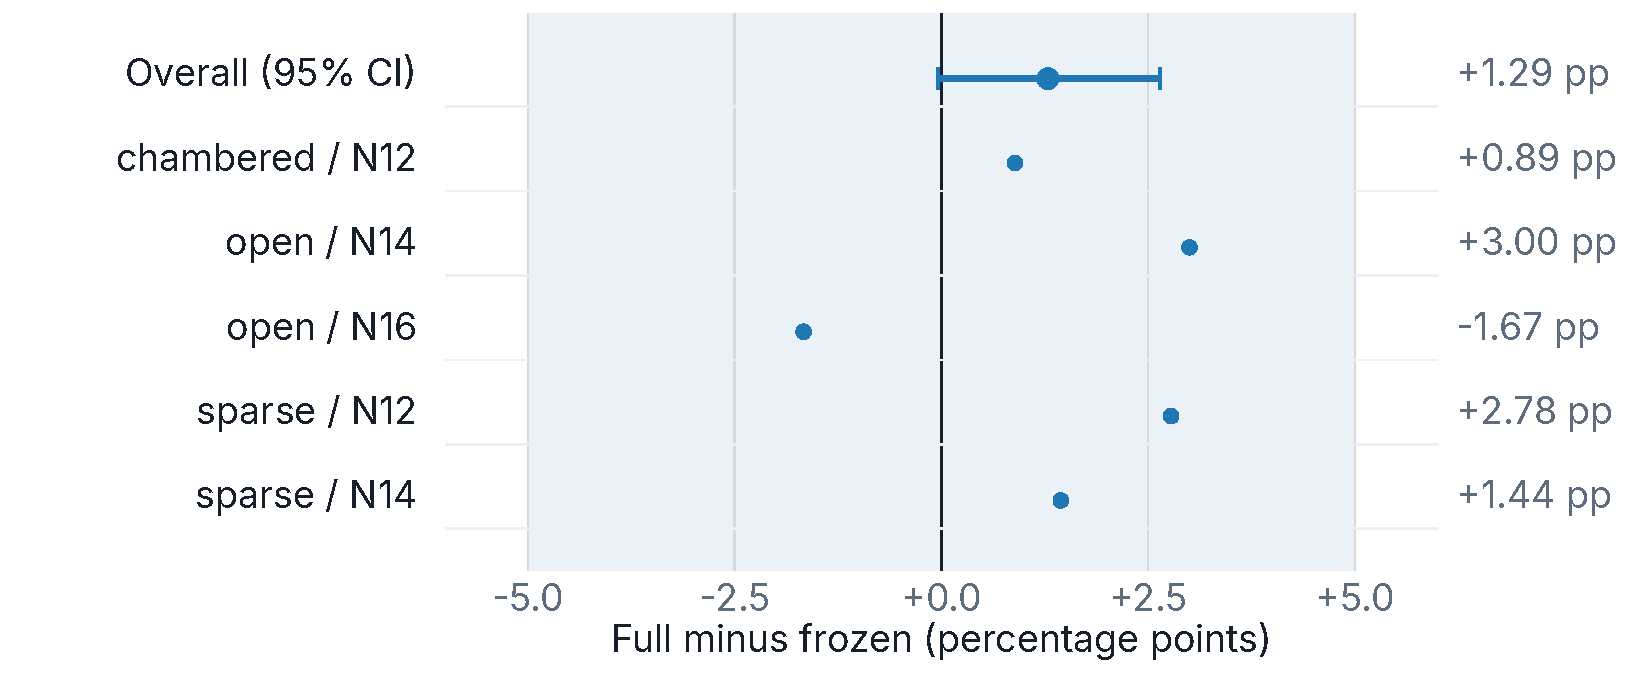
\includegraphics[width=\textwidth]{Fig1.pdf}
\caption{Full-minus-frozen solve-probability effects. The overall interval is the prespecified stratified puzzle-bootstrap interval. Only point estimates are shown for strata; these are descriptive. The shaded band marks \(\pm\)5 percentage points}\label{fig-primary}
\end{figure}

The five descriptive stratum effects ranged from \(-\)1.67 points for open 16\(\times\)16 to +3.00 points for open 14\(\times\)14 (Table~\ref{tab-strata}). No stratum point estimate crossed either practical boundary. These estimates were not separately powered or multiplicity-adjusted and should not be read as evidence of family-specific benefit. Descriptively, the larger positive estimates fell in strata with mid-to-high base solve rates (open 14\(\times\)14 and sparse 12\(\times\)12, near 0.67 and 0.74), while the hardest strata (open 16\(\times\)16 and sparse 14\(\times\)14, near 0.29 and 0.16) showed a small negative and a small positive estimate.

\begin{table}[htbp]
\centering
\caption{Predeclared descriptive results by generator stratum. Each row contains 30 puzzles, 30 seeds per puzzle, and 900 trials per condition}\label{tab-strata}
\begin{tabular}{lrrr}
\toprule
Stratum & Full & Frozen & Difference \\
\midrule
Chambered, 12\(\times\)12 & 0.379 & 0.370 & +0.009 \\
Open, 14\(\times\)14 & 0.684 & 0.654 & +0.030 \\
Open, 16\(\times\)16 & 0.279 & 0.296 & \(-\)0.017 \\
Sparse, 12\(\times\)12 & 0.753 & 0.726 & +0.028 \\
Sparse, 14\(\times\)14 & 0.170 & 0.156 & +0.014 \\
\bottomrule
\end{tabular}
\end{table}

Across the 4,500 paired puzzle-seed combinations, both arms solved 1,574, only full feedback solved 465, only frozen feedback solved 407, and neither solved 2,054. At puzzle level, full feedback had a higher seed solve rate on 57 puzzles, the arms tied on 48, and frozen feedback was higher on 45. The distribution of per-puzzle effects is heterogeneous but centered near zero (Fig.~\ref{fig-puzzles}); the secondary displays do not alter the primary classification. Thirty-six of the 150 puzzles were solved identically by both arms on every seed (13 by neither arm and 23 by both), so their observed per-puzzle differences are zero. They remain part of the 150-puzzle target population and contribute to its denominator and bootstrap uncertainty. Excluding these puzzles gives a mean difference of +1.70 percentage points across the remaining 114 puzzles, but selects a subset using observed outcomes and changes the target population. This post-hoc descriptive calculation has no accompanying interval and does not establish equivalence for that subset; the confirmatory estimate retains all 150 puzzles.

\begin{figure}[htbp]
\centering
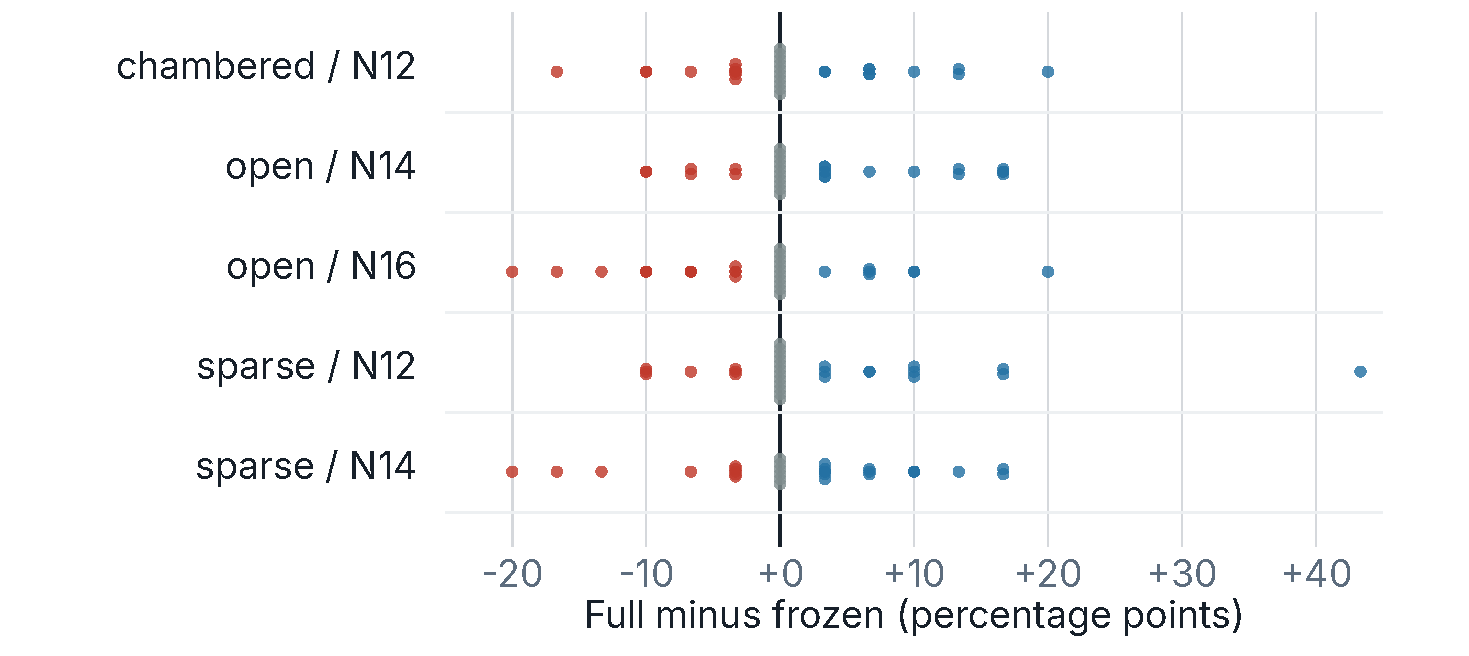
\includegraphics[width=\textwidth]{Fig2.pdf}
\caption{All 150 per-puzzle differences, sorted within stratum. Positive values favor full feedback, negative values favor frozen feedback, and zero denotes a tie; position relative to zero conveys direction independently of color. This plot is descriptive}\label{fig-puzzles}
\end{figure}

\section{Discussion}

The controlled result is negative in the scientifically useful sense: the implemented edge-feedback package did not produce a practically important average improvement under the frozen Challenge v1 design. The point estimate favors feedback slightly, but the full 95\% interval (from a negligible disadvantage to a 2.64-point advantage) remains well inside the \(\pm\)5-point band. The interval includes zero and small positive effects. Its containment within the predeclared band supports practical equivalence for the studied average effect, without establishing that feedback is exactly neutral. Describing this result only as ``not significant'' would miss the predeclared practical claim; describing it as universal equivalence would overstate it.

The result clarifies the legacy ceiling. On the original test corpus, the tuned full constructor solved 1,110/1,110 trials, and a post-hoc same-configuration frozen diagnostic also solved 1,110/1,110. Challenge v1 lowered both methods into an informative success regime, yet the average contrast remained small. Together, these observations suggest that the constraint-aware constructor, not its adaptive edge state, is the dominant source of performance in the studied settings.

Several mechanisms could explain the small contrast. First, hard residual-connectivity pruning is powerful: it removes moves that would make Hamiltonian completion impossible. Second, the onward-degree heuristic directly encodes a classic constructive principle, while waypoint legality and parity balance further narrow the choice set. Third, the relatively high edge-replacement probability ($z=0.3879$ independently per edge per update) can disrupt accumulated state as well as diversify it. Finally, 64 iterations may be sufficient for the constructor to sample many useful paths but too short, too long, or otherwise mismatched for stable edge learning. The present intervention intentionally does not decide among these explanations. In particular, because $z$ and $\tau_{\max}$ were fixed by legacy full-feedback tuning (where they were only weakly identified) and were never optimized for the Challenge contrast, the near-null result cannot separate an intrinsically inert feedback signal from a real but miscalibrated one that a different replacement rate, clip, or iteration cap might render useful. The ablation answers whether this configured update helps, not whether edge feedback can be made to help.

Methodologically, the study illustrates why mechanism ablations should preserve the surrounding algorithm. A separate ``heuristic baseline'' with a different population or budget cannot identify the effect of feedback. Freezing a zero-initialized state inside the same implementation removes a much narrower component. Likewise, a hard benchmark selected because the proposed method wins can bias the treatment contrast. Challenge v1 used only frozen-arm difficulty for calibration and concealed the confirmatory split until the analysis was immutable.

The practical-equivalence band is a scientific judgment rather than a fact supplied by the data. Five percentage points was chosen before unlock as the smallest average solve-probability gain that would justify retaining the update's machinery (signed rank deposition, temporal decay, and per-edge stochastic replacement, together with the extra hyperparameters ($\alpha$, $z$, $\tau_{\max}$) and the per-iteration rank sort and whole-edge-set deposit they impose) over the simpler stateless constructor; a smaller average gain would not, in our judgment, warrant that added complexity and tuning burden for this endpoint. Readers who prefer a narrower threshold can still use the reported interval: it rules out average improvements above 2.64 points at the chosen confidence level but does not establish equivalence inside, for example, \(\pm\)1 point. Reporting the estimate and interval keeps that sensitivity visible.

The outcome does not imply that shared edge memory has no research value. Heterogeneous effects and the mechanistic structure motivate new, explicitly exploratory work: separately remove rank-negative deposits, decay, and edge replacement; vary the construction budget; learn state per waypoint segment; or identify instance features that modify the effect. Such studies should use new development data and a newly locked confirmatory split. They should not repurpose the released Challenge v1 test set for another confirmatory claim.

\section{Limitations and threats to validity}

\textbf{Synthetic instances.} Challenge v1 guarantees solvability and avoids third-party data rights, but its instances arise from one planted-certificate generator. Backbite-randomized paths, deceptive waypoint placement, and certificate-preserving walls may not represent human-authored puzzles or other Hamiltonian graph distributions.

\textbf{Limited domain and scales.} The confirmatory set covers five family/size strata and square grids of size 12, 14, or 16. Conclusions may not generalize to larger grids, blocked cells, non-grid graphs, other waypoint densities, or different wall processes.

\textbf{One configuration and budget.} The heuristic and feedback hyperparameters were inherited from the legacy tuned winner rather than re-tuned on Challenge v1, and that winner was selected where both arms saturated near a solve ceiling; only the iteration cap (hence the 3,392-path budget) and the five strata were set from feedback-frozen development difficulty. The experiment therefore estimates the effect of feedback at this transported operating point, not one chosen to make feedback maximally useful, and it neither averages over hyperparameters nor shows that either arm is optimally tuned. Re-tuning each arm on development solve rate (which does not select on the treatment contrast) could give feedback a stronger chance and is left to explicitly exploratory work. Interactions between feedback and population, iteration cap, state clipping, or noise may change the effect.

\textbf{Composite intervention.} Freezing the update simultaneously removes signed rank deposits, temporal decay, and stochastic edge replacement. The design has strong isolation at the package level but cannot attribute the result to a subcomponent. The nonnegative state also clips negative aggregate deposits; calling it ``positive-only'' would be inaccurate.

\textbf{Random-stream divergence.} Conditions share their initial derived seed, but feedback consumes random draws, so their streams cease to be synchronized. The comparison is between two stochastic algorithms with paired initialization, not a common-random-number estimate at every construction decision.

\textbf{Practical band and interval.} The \(\pm\)5-point band was predeclared but remains domain judgment. The empirical percentile cluster bootstrap is transparent and reproducible, but other interval procedures could differ in finite samples. The classification is not a formal TOST result.

\textbf{No state-of-the-art comparison.} The mechanism question requires a matched constructor ablation, not a leaderboard. This paper therefore does not establish superiority over exact solvers, constraint programming, specialized ACO, or other tuned metaheuristics. Archived legacy baselines are contextual only and are not used for the confirmatory claim.

\section{Reproducibility and data availability}

The software, benchmark specification, public train/development corpus, test commitment, frozen protocol, and analysis are included with the artifact. The pre-test release is Git commit \path{06ef8bbfae5de29fe6cd4ebf0175a94f04880e9b} and annotated tag \path{challenge-v1-confirmatory-v1}. The post-analysis evidence directory contains all 9,000 raw rows, 4,020 solved coordinate paths, the exact test corpus and certificates, the revealed seed, 10,000 bootstrap replicates, per-puzzle effects, environment and hardware metadata, and SHA-256 checksums.

The raw result SHA-256 is \path{a899646ef363ad2fd295e704b35f73b22efeb08ad10ebd5dc6429e1d32b1976a}. Execution used Python 3.13.12, NumPy 2.4.4, Numba 0.65.1, and Polars 1.40.1 on an AMD Ryzen 9 9950X3D system with 32 logical CPUs. The complete 9,000-run grid finished in 145.0 seconds with no failed rows; timing is provenance, not a comparative endpoint.

From the repository root, \path{make paper-verify} checks the frozen protocol, \path{make paper-smoke} exercises both arms on public data, \path{make paper-analyze} regenerates the analysis, and \path{make paper-figures} regenerates publication displays. For audit from the paper package alone, \path{paper/scripts/secondary_analysis.py} re-derives the primary interval from the archived per-puzzle effects, reproducing the frozen 10,000-replicate bootstrap byte for byte, and regenerates the post-hoc descriptive quantities (achieved precision, saturation counts, and the outcome-selected subset calculation) reported above. The evidence package documents seed reconstruction and byte-level verification. The public repository is available at \url{https://github.com/gtkacz/zipmould}, and the accompanying evidence package contains the released data and analysis artifacts. A versioned archival deposit is being prepared before journal submission.

\section{Conclusion}

ZipMould's edge-state feedback was tested against the same stochastic constructor with the update frozen, under a sealed and reproducible Challenge v1 protocol. Full feedback improved average solve probability by 1.29 percentage points, with a 95\% puzzle-bootstrap interval from \(-\)0.04 to +2.64 points. This interval lies within the predeclared \(\pm\)5-point band, yielding a practically equivalent classification. The evidence therefore supports a narrow conclusion: for this implementation, benchmark, configuration, and budget, adding adaptive edge feedback produced no practically important average gain over the stateless constructor, while remaining compatible with a small positive effect. Publishing that result, together with the test commitment, raw paths, and exact analysis, provides a firmer basis for future mechanism design than attributing ceiling performance to a biological metaphor.

\section{Statements and Declarations}

\textbf{Ethics approval:} Not applicable; the study uses synthetic benchmark instances and no human or animal participants.

\textbf{Funding:} This study was financed in part by the Coordena\c{c}\~{a}o de Aperfei\c{c}oamento de Pessoal de N\'{i}vel Superior -- Brasil (CAPES) -- Finance Code 001, and in part by the Conselho Nacional de Desenvolvimento Cient\'{i}fico e Tecnol\'{o}gico -- Brasil (CNPq). The work received no dedicated project funding beyond these graduate scholarships.

\textbf{Competing interests:} The authors declare that they have no competing interests.

\textbf{Acknowledgements:} This work was developed as part of the first author's Master of Engineering at Mackenzie Presbyterian University.

\textbf{AI assistance:} OpenAI Codex assisted with manuscript assessment, statistical wording revisions, LaTeX conversion, and submission-package preparation. The underlying confirmatory results were retained, and the archived analysis was regenerated to check consistency.

\bibliography{references}
\end{document}
